\section{Application}
\label{sec:application}

This section applies the frozen design to an external benchmark: the Tennessee Eastman Process (TEP)
of \citet{downs_plant_wide_1993}, a simulated closed-loop chemical plant with a reactor, separator and stripper under feedback control, in the extended version released by \citet{reinartz_extended_2021} as a fault-detection benchmark. Its faults have known onsets and severities, so detection can be timed against the truth, and its purpose here is to test whether the frozen design transfers to a larger closed-loop process. It is a simulation, not measured plant data, and the synthetic study remains the primary experiment.

\subsection{Benchmark and frozen protocol}

In Mode~1, the data are sampled every 3 minutes and are nominal until the fault activates after
30 hours \citep{reinartz_tennessee_2021}. The fault is the process disturbance IDV(2): a step in the
B composition of feed stream~4, with the ratio of components A and C (A/C) held
constant \citep{reinartz_extended_2021}, at severities of 25, 50, 75 and 100\%. The 31 variables
($p=31$) under consideration are the 22
continuous measurements and the nine non-constant manipulated variables. Whole runs are allocated to
roles: nominal pre-fault segments of other runs form TEP-D1 to TEP-D4, in the roles of D1--D4, and
TEP-D5 comprises all 500 IDV(2) runs (Appendix~\ref{app:tep}).

$H(0.05)$ and $M(0.05)$ follow the guidelines of Sections~3.2--3.3, with $L=32$,
$q=8$, $\nu=0.03$ and $\lambda=0.05$. Only the CAE's channel count changed, and every component was
refitted on TEP Phase~I data and frozen before TEP-D4 and TEP-D5 were read, without tuning. The
dataset contains only five independent long nominal runs, so an $\ARL_0$ of 370 cannot be estimated.
Each limit instead gives a 5\% probability of at least one false alarm over the 568 nominal
decisions, and no \ARL{} equivalent is claimed.

To evaluate the delay in fault detection, each chart runs from the start of the simulation without restarts, and a run is
eligible for a chart if that chart gave no alarm before onset. The onset-referenced conditional
detection delay $D$ counts decisions from onset to the first signal ($D=1$ at 30.00~h; $0.05(D-1)$ hours
elapsed; censoring at $D=1401$). $H$ and $M$ are compared on jointly eligible runs with the paired
estimator of Equation~(\ref{eq:paired}); a positive $D_H-D_M$ means that the hybrid chart was slower.
Because $D$ follows IC operation and conditions on no earlier alarm, it is not an $\ARL_1$,
and severity is not comparable with $\delta$. The hybrid chart's window at delay $D$ holds only
the smaller of $D$ and 32 post-change observations, whereas $M$ sees the change from $D=1$.

\subsection{Results and interpretation}

On TEP-D4 the false-alarm probability was 0.0435 for $H(0.05)$ and 0.0425 for $M(0.05)$ (exact 95\%
intervals 0.035--0.053 and 0.034--0.052), and before onset in TEP-D5 it was 0.036 and 0.038. Both
charts therefore met the criterion and, unlike in Section~4.2, were matched in the IC state. Delays fell monotonically with severity (Figure~\ref{fig:tep}; medians in Table~\ref{tab:tep}), and $M(0.05)$ was faster at every severity. The mean paired differences $D_H-D_M$ ranged from
$+10.1$ to $+4.8$ decisions (about 0.51 to 0.24~h), each many standard errors above zero, and the hybrid chart was slower in every jointly eligible run at 25--75\% and in 185 of 188 at 100\%.

Part of the gap is structural: at 50--100\% every eligible
hybrid signal came before its window was entirely post-change ($D<32$), and only at 25\% did its
median delay (39) come later. The criterion bounds false alarms only over the 568 nominal decisions,
although all delays (7--49 decisions) fell well within the 1401-decision horizon. The 100\% cell is confounded with a separate seed batch, which
showed no consistent IC batch effect, and only IDV(2) was evaluated (see Figure~\ref{fig:tep}).

\begin{table}[!ht]
\centering
\caption[Detection delays in the Extended TEP application]{Extended TEP, IDV(2):
onset-referenced conditional detection delay $D$ in monitoring decisions of 3~min (elapsed hours
$0.05(D-1)$ in parentheses) and the numbers of runs eligible for $H(0.05)$, $M(0.05)$ and both.
Eligibility requires no pre-onset alarm; a positive $D_H-D_M$ means that the hybrid chart was slower. No
eligible delay was censored.}
\label{tab:tep}
\begin{tabular}{lrcrrr}
\toprule
 & & Eligible & \multicolumn{2}{c}{Median $D$ (hours)} & Paired mean \\
\cmidrule(lr){4-5}
Severity & Runs & $H$/$M$/paired & $H(0.05)$ & $M(0.05)$ & $D_H-D_M$ (SE) \\
\midrule
\tabinput{tables/tep_d5_primary.tex}
\bottomrule
\end{tabular}
\end{table}

\begin{figure}[!ht]
\centering
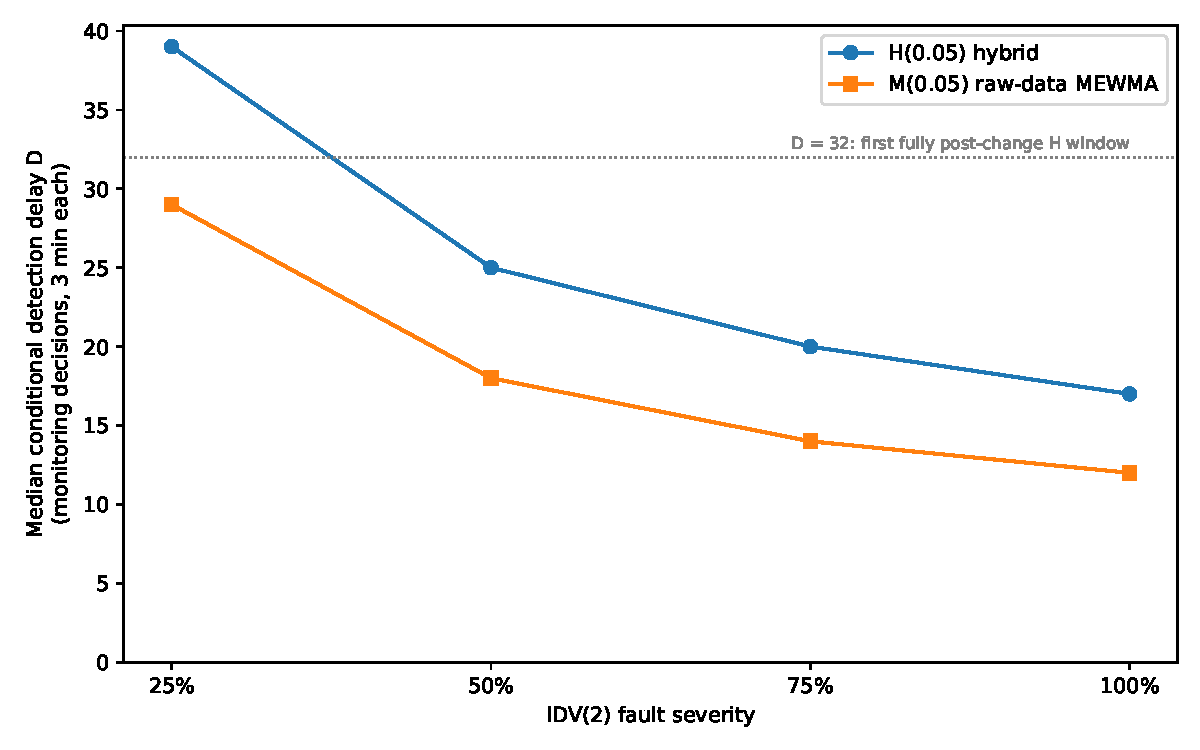
\includegraphics[width=0.9\linewidth]{tep_d5_median_delay.pdf}
\caption[Median detection delay against IDV(2) severity]{Extended TEP, IDV(2): onset-referenced
conditional detection delay. Median onset-referenced conditional
detection delay of $H(0.05)$ and $M(0.05)$ against IDV(2) severity (eligible runs of
Table~\ref{tab:tep}); the dotted line marks $D=32$, the first entirely post-change hybrid window.}
\label{fig:tep}
\end{figure}

The frozen framework thus transfers, calibrates to a horizon-appropriate criterion and responds coherently to the fault, but shows no advantage over the classical chart. IDV(2) is a persistent step disturbance, which a raw-data MEWMA accumulates
efficiently \citep{lowry_multivariate_1992}, and the ordering matches the primary comparison.
Because the onset followed 568 IC decisions, the startup mechanism of Section~4.5 cannot
explain this gap, although the ramp-in can explain part of it. Deployment would also need a genuinely IC reference period and refitting after legitimate process changes, and its signals are harder to attribute to variables than those of a raw-data MEWMA, whose state vector shows the shift direction \citep{lowry_multivariate_1992}.
